\section{Methodology} \label{sec:model}
A challenge in applying truth discovery to community discussion forums is capturing the diversity of user's knowledge and the diversity of word usage in the answers. To address it, we model user-aspect reliability and learn semantic representations of the comments.
\subsection{Problem Formulation}
Each \textit{submission} is a post, i.e., question, which starts a discussion thread while a \textit{comment} is a response to a submission post.
Formally, each submission post, $m$, is associated with a set of terms, $c_m$. A user, $n$, may reply with a comment on submission $m$, with a set of terms $w_{m, n}$. $\mathcal{V}$ is the vocabulary set comprising of all terms present in our dataset i.e. all submissions and comments. Each term, $\omega \in \mathcal{V} $ has a corresponding word-vector representation, or word embedding, $\bm{v}_\omega \in \mathbb{R}^D$. Thus, we can represent a \emph{post embedding} in terms of its constituent terms, $ \{ \bm{v}_c \}, \forall c \in c_m $. To capture the semantic meaning, we represent each comment as the mean word-vector representation of their constituent terms\footnote{Sentence, and furthermore document representation is a complex problem. In our work, we explore a simple aggregation method for comment semantic composition ~\cite{wang2016sentence}.}. Formally,
we represent the comment given on the post $m$ by user $n$ as the \emph{comment embedding}, $\bm{a}_{m,n} = {\vert w_{m, n} \vert}^{-1} \sum_{\omega \in w_{m,n}} \bm{v}_{\omega}$. Our model treats the post embeddings as static and learns the comment word embeddings. The set of posts user $n$ has commented on is denoted by $\mathcal{M}_n$ and the set of users who have posted on submission $m$ is denoted as $\mathcal{N}_m$.

There are $K$ aspects or topics discussed in the forum, and each post and comment can be composed of multiple \emph{aspects}. We denote submission $m$'s distribution over these aspects as the \emph{post-aspect distribution}, $\bm{p}_m \in \mathbb{R}^K$.
Similarly, we also compute, \emph{user-aspect distribution}, $\bm{u}_n \in \mathbb{R}^K$, learned over all the comments posted by the user $n$ in the forum. This distribution captures familiarity (or frequency) of user $n$ with each aspect based on their activity in the forum. Each user $n$ also has a \emph{user reliability} vector defined over $K$ aspects, $\bm{r}_n \in \mathbb{R}^K$.
The reliability captures the likelihood of the user providing a trustworthy comment
about a specific aspect. Note high familiarity in an aspect does not always imply high reliability in the same aspect. Table \ref{tab:symbols} presents all the symbols and their meanings.

For each submission post $m$ associated with a set of responses $\{ \bm{a}_{m,n} \}$, our goal is to estimate the real-valued vector representations, or \emph{latent trustworthy comment} embeddings, $\bm{a}_m^* \in \mathbb{R}^D$. We also simultaneously infer the \emph{user reliability} vector $\{\bm{r}_n\}$ and update the word embeddings $\{\bm{v}_{\omega}\}$. The latent trustworthy comment embeddings, $\bm{a}_m^*$, can be used to rank current comments on the post.

\begin{table}[tbh]
  \centering
\begin{tabular}{c l} \toprule
Notation              & Definition \\
\midrule
$\mathcal{V}$ &  vocabulary associated with submission/comments \\
$\mathcal{M}_n$ & submissions where user $n$ has commented \\
$\mathcal{N}_m$ &  users who have commented on submission $m$ \\
$\mathcal{D}_{\omega}$ &  comment-submission pairs where $\omega$ term appears \\
$c_m$       & set of terms associated with submission post $m$ \\
$v_{\omega}$    & word embedding for term $\omega$\\
$a_{m, n}^{-\omega}$    & aggregate embedding of terms in $w_m^n$ excluding term $\omega$\\
$a_{m, n}$    & embedding of the comment from user $n$ on post $m$\\
$a_{m}^{*}$    & embedding of the latent trustworthy comment for post $m$\\
$u_{n}^{(k)} $     & $k$th aspect weight for user $n$ \\
$p_{m}^{(k)} $     & $k$th aspect weight for submission post $m$ \\
$r_n^{(k)}$   & learned user-aspect reliability for user $n$ for aspect $k$\\
$R_m^n$     & the user-post reliability for the $n$th user and the $m$th post \\
$M$     & total number of posts \\
$N$     & total number of users \\
\bottomrule
\end{tabular}
\caption{Symbols and their meaning}
\label{tab:symbols}
\end{table}

\subsection{Proposed Method}
Our model follows the truth discovery principle: trustworthy comment is supported by many reliable users and vice-versa. In other words, the weighted error between the trustworthy comment and the given comments on the post is minimum, where user reliabilities provide the weight. We extend the approach to use an aspect-level user reliability and compute a post-specific reliability weight.
We further compute the error in terms of the \textit{embeddings} of posts and comments to capture their semantic meaning.

In particular, we minimize the \emph{embedding error}, $E_{m,n} = \vert \vert \bm{a}_m^* - \bm{a}_{m,n} \vert \vert^ 2$, i.e., mean squared error between learned \emph{trustworthy comment} embeddings, $\bm{a}_m^*$ and comment embeddings, $\bm{a}_{m,n}$, on the post $m$. This error ensures that the trustworthy comment is semantically similar to the comments given for the post.

Next, to ensure context similarity of the comments with the post, we compute the \emph{context error}, $Q_{m,n}= \vert c_m \vert^{-1} \sum_{c \in c_m} \vert \vert \bm{a}_{m,n} - \bm{v}_c \vert \vert^2$, reducing the difference between the \emph{comment embeddings} and \emph{post embeddings}. The key idea is similar to that of the distributional hypothesis that if two comments co-occur a lot in similar posts, they should be closer in the embedding space.

Further, these errors are weighted by the aspect-level reliability of the user providing the comment.
We estimate the reliability of user $n$ for the specific post $m$ through the \emph{user-post reliability} score, $R_{m,n} = \bm{r}_n \odot s(\bm{u}_{n}, \bm{p}_{m}) = \sum_{k} \bm{r}_n^{(k)} \cdot (\bm{u}_{n}^{(k)} \cdot \bm{p}_{m}^{(k)} )$. The $\odot$ symbol represents the Hadamard product. This scores computes the magnitude of \emph{user reliability} vector, $\bm{r_n}$, weighted by the similarity function $s(.)$.
The similarity function $s(\bm{u}_{n}, \bm{p}_{m})$ captures user familiarity with post's context by computing the product of the aspect distribution of user $n$ and post $m$.
Thus, to get a high \emph{user-post reliability} score, $R_{m,n}$, the user should both be reliable and familiar to the aspects discussed in the post.

Finally, these errors are aggregated over all the users and their comments.
Thus, we define our objective function as follows,
\begin{equation}
\resizebox{0.75\textwidth}{!}{$
\begin{aligned}
\underset{\{\bm{a}_m^{*}\}, \{\bm{v}_{\omega}\}, \{\bm{r}_n\} }{ \text{min}}
\sum_{n=1}^{N} \sum_{m \in \mathcal{M}_n} \underbrace{R_{m,n}}_{\text{user-post reliability}} \left( \underbrace{E_{m,n}}_{\text{embedding error}} + {\beta} \odot \underbrace{Q_{m,n}}_{\text{context error}} \right) \\
 \text{s.t. } \sum_{n=1}^N e^{-\bm{r}_n^{(k)}} = 1; \forall k
\end{aligned}
$}
\end{equation}
where $N$ is the number of users. $ R_{m, n} \cdot E_{m,n}$ ensures that the latent trustworthy comment embeddings are most similar to comment embeddings of \emph{reliable} users for post $m$. While $ R_{m,n} \cdot Q_{m,n}$ ensures trust aware learning of contextualized comment embeddings. The hyperparameter $\beta$ controls the importance of context error in our method. The exponential regularization constraint, $\sum_{n=1}^N e^{-\bm{r}_n^{(k)}}=1$ for each $k$, ensures that the reliability across users are nonzero. Figure \ref{fig:model} shows the overview of our model using a toy example of a post in a medical forum with flu-like symptoms. The commenters describing flu-related diagnoses are deemed more reliable for this post.

\begin{figure}[tb]
\centering
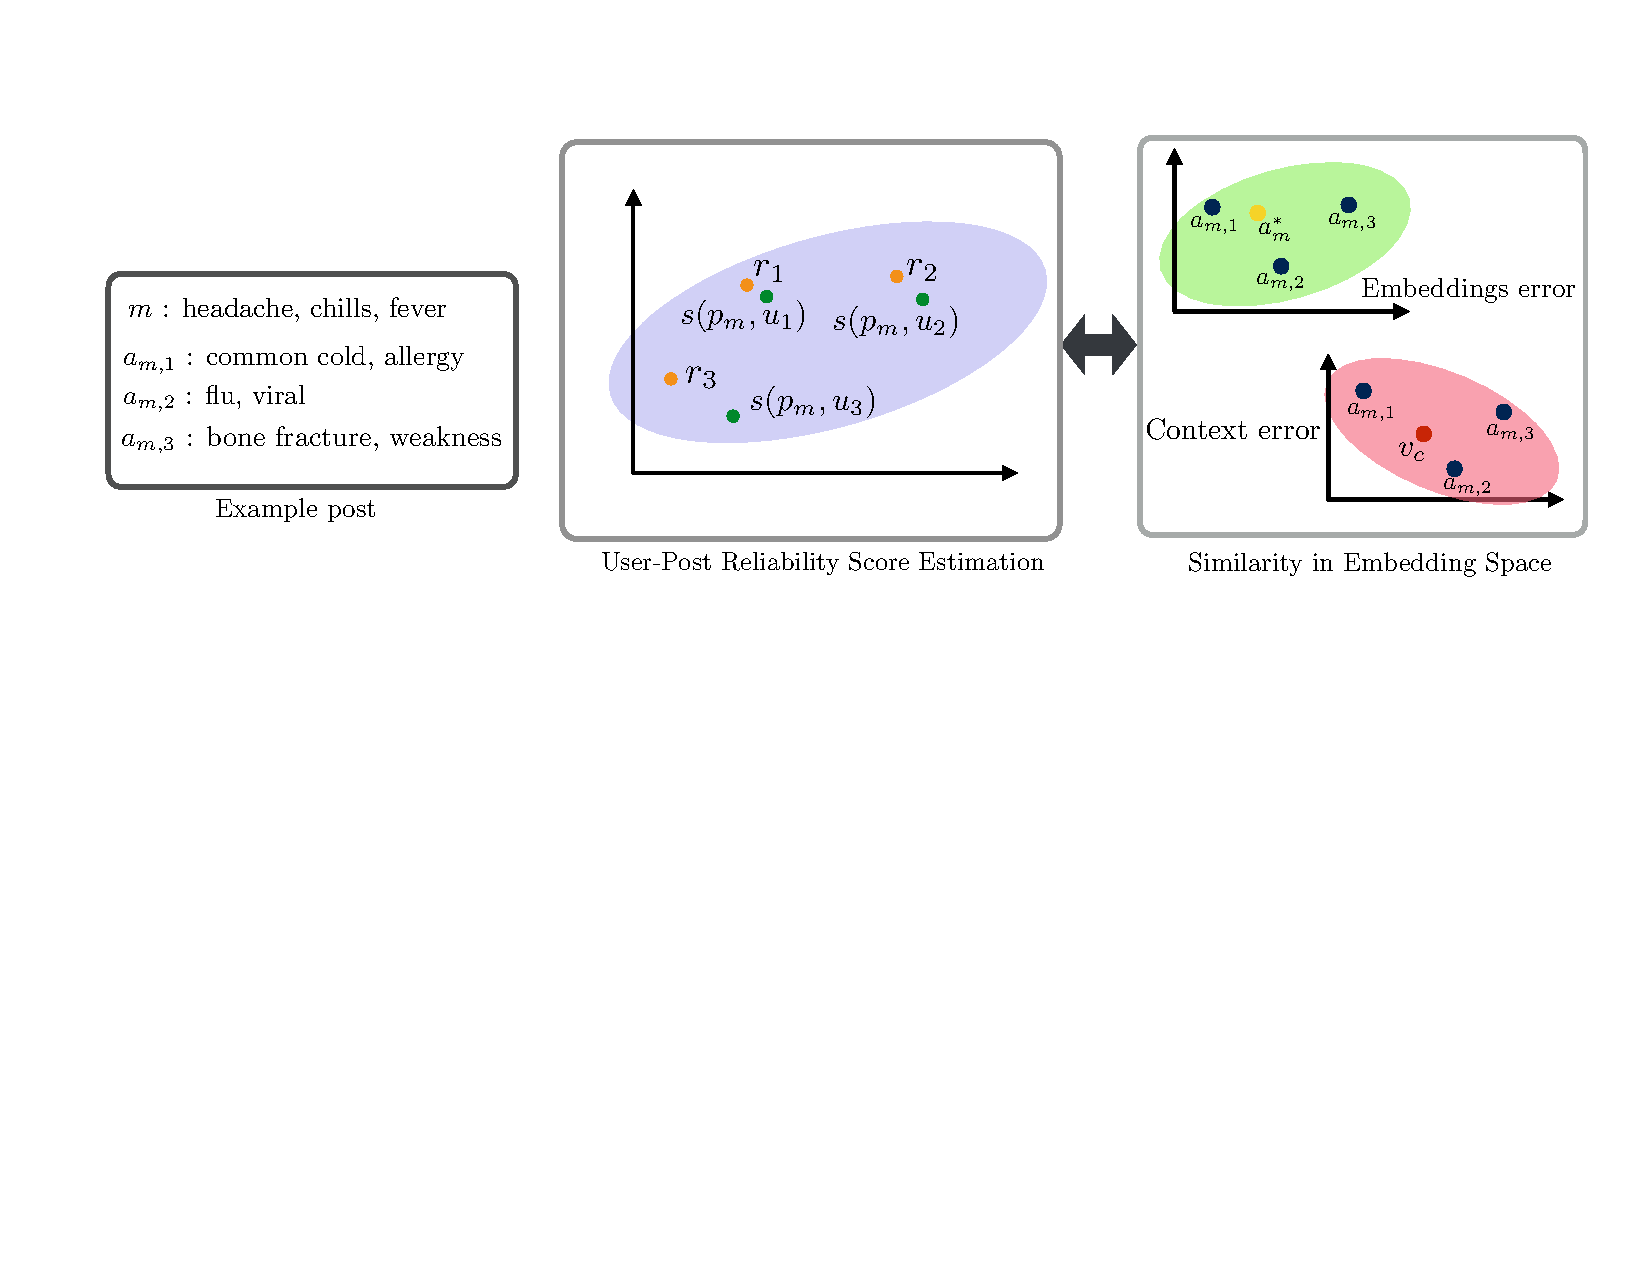
\includegraphics[scale=0.6]{images/architecture_gray_post_combined.pdf}
\caption{\small An illustrative toy example detailing our model components.
The left-hand side details the user-post reliability score estimation, $R_{m,n}$, that is a function of similarity function $s(.)$ between the user and post aspect distributions and user aspect reliabilities, $\bm{r}_n$. In the right-hand, we learn trustworthy comment embedding, $\bm{a}_m^{*}$, such that it is similar to user comments, $\bm{a}_{m,n}$ which are, in turn, similar to the post context $\bm{v}_c$.
}
\label{fig:model}
\end{figure}

\subsection{Solving the Optimization Problem}
We use coordinate descent \cite{bertsekas1999nonlinear} to solve our optimization problem. In particular, we solve the equation for each variable while keeping the rest fixed.

\paragraph{Case 1:}
Fixing $\{\bm{r}_n\}$ and $\{ \bm{v}_{\omega} \}$
, we have the following update equation for $ \{ \bm{a}_m^* \}$:
 {\small
\begin{align}
\bm{a}_m^* = \frac{ \sum_{n \in \mathcal{N}_m} R_{m,n} \bm{a}_{m,n} } { \sum_{n \in \mathcal{N}_m} R_{m,n} }
\end{align}
}
Thus, the latent \emph{trustworthy comment} is a weighted combination of comments where weights are provided by the \emph{user-post reliability} score $R_{m,n}$.
Alternatively, it can also be interpreted as a reliable summarization of all the comments.
\paragraph{Case 2:}
Fixing $\{ \bm{a}_m^* \}$, $\{ \bm{v}_{\omega} \}$
, we have the following update equation for $ \{\bm{r}_n^{(k)}\}$:
\begin{equation}
\resizebox{0.55\linewidth}{!}{$
\begin{aligned}
\bm{r}_n^{(k)} \propto - \ln {\sum_{m \in \mathcal{M}_n} s(\bm{u}_{n}^{(k)} , \bm{p}_{m}^{(k)}) \left( E_{m,n} + {\beta } Q_{m,n} \right)}
\end{aligned}
$}
\end{equation}
Reliability of a user in aspect $k$ is inversely proportional to the errors with respect to the latent trustworthy comment $\bm{a}_m^{*}$ ($E_{m,n}$) and submission's context $\bm{v}_c$ ($Q_{m,n}$) over all of her posted comments ($\mathcal{M}_n$). The embedding error ensures that if there is a large difference between the user's comment and the trustworthy comment, her reliability becomes lower. The context error ensures that non-relevant comments to the post's context are penalized heavily. In other words, a reliable user should give trustworthy and contextualized responses to posts.

This error is further weighed by the similarity score, $s(.)$, capturing familiarity of the user with the post's context. Thus, familiar users are penalized higher for their mistakes as compared to unfamiliar users.

\paragraph{Case 3:}
Fixing $\{ \bm{a}_m^* \}, \{\bm{r}_n^{(k)}\}$,
we have the following update equation for $\{ \bm{v}_{\omega} \}$:
\begin{equation}
\resizebox{.85\hsize}{!}{$
\begin{aligned}
 \bm{v}_{\omega} &= \frac{\sum_{<m,n> \in D_{\omega}} R_{m,n}\left( \bm{a}_m^* + \beta \vert c_m \vert^{-1} \sum_{c \in c_m} \bm{v}_c \right)
 - R_{m,n} (\beta + 1)\vert c_m \vert^{-1} \bm{a}_{m,n}^{- \omega} }{ \sum_{<m,n> \in D_{\omega}} R_{m,n}(\beta + 1)}
\end{aligned}
$}
\end{equation}
where $<m,n> \in D_{\omega} = \{ (m,n) \vert \omega \in w_{m,n} \}$ and $\bm{a}_{m,n}^{-\omega} = \vert w_{m, n} \vert^{-1} \sum_{\omega' \in w_{m,n} \setminus \{ \omega \} } \bm{v}_{\omega'}$. To update $\bm{v}_\omega$, we only consider those comment and submission pairs, $D_{\omega}$, in which the particular word appears.
The update of the embeddings depend on the submission context $\bm{v}_c$, latent trustworthy comment embedding, $\bm{a}_m^*$ as well as \emph{user-post reliability} score, $R_{m,n}$. Thus, word embeddings are updated in a trust-aware manner such that reliable user's comments weigh more than those of unreliable users as they can contain noisy text. Note that there is also some negative dependency on the contribution of other terms in the comments.

\noindent
\textbf{Implementation Details:}
We used popular Latent Dirichlet Allocation (LDA)~\cite{blei2003latent} to estimate aspects of the posts in our dataset\footnote{We ran LDA with 50 topics for all experiments and examined its sensitivity in Section \ref{Results}.}. Specifically, we combined the title and body text to represent each post. We applied topic model inference to all comments of user $n$ to compute its combined aspect distribution, $\bm{u}_n$.
We randomly initialized the user reliability, $\bm{r}_n$. We initialized the word embeddings, $\bm{v}_\omega$, via word2vec~\cite{mikolov2013distributed} trained on our dataset. We used both unigrams and bigrams in our model. We fixed $\beta$ to $0.15$.\footnote{We did not find a significant change in results for different values of $\beta$.}
The model converges after only about six iterations indicating quick approximation.
In general, the computational complexity is $O(\vert \mathcal{V} \vert N M)$; however,
we leverage the data sparsity in the comment-word usage and user-posts for efficient implementation.
